\chapter{Imaging}\label{c:imaging}

\section{Detector Cuts} \label{sec:ch8-det-cuts}

Approximately xxx \% of the detectors in the array can not be used to generate images.
For some, the detector membranes are broken.
Others appear intact upon visual inspection, but show no response to applied current even in the superconducting state.
Others work as expected while superconducting, but can not be biased so as to show a response to changes in optical power. 
And some are extremely noisy or consistently show other problems in the data stream.
This section summarizes which detectors have each of these problems.
\figref{fig:detector-cuts-wafer} and \figref{fig:detector-cuts-rc} contain plots summarizing this information graphically, organized by detector position on the wafer and by readout row/column respectively.

To determine which detectors show no response in the superconducting state, the temperature of the focal plane was set to 975~mK, well below the $T_c$ of the detectors.
The \TES\ bias current was ramped, and data was acquired while running the readout system open-loop.
\figref{fig:tes-bias-ramp-sc} shows the resulting data for rows 0 -- 4 of all columns.
Most row/column combinations show a response that maps out the $V$-$\Phi$ curve for the SQUID amplifier chain.
The row/column combinations that show no response indicate either a broken detector line, a broken SQUID on a mux chip, broken wirebonds, or some other problem in the readout system.

Another group of detectors remain superconducting at the chosen bias point and operating temperature of 1100~mK.
This could be caused by an abnormally high $G$ value, or by a short somewhere in the \TES\ circuit.
\figref{fig:tes-bias-ramp-trans} shows the result of ramping \TES\ bias current while running the readout system open-loop, but while the system is at 1100~mK and the \TESs\ are biased into the transition at a DAC value of 27000.

\begin{figure*}[th]
\centering
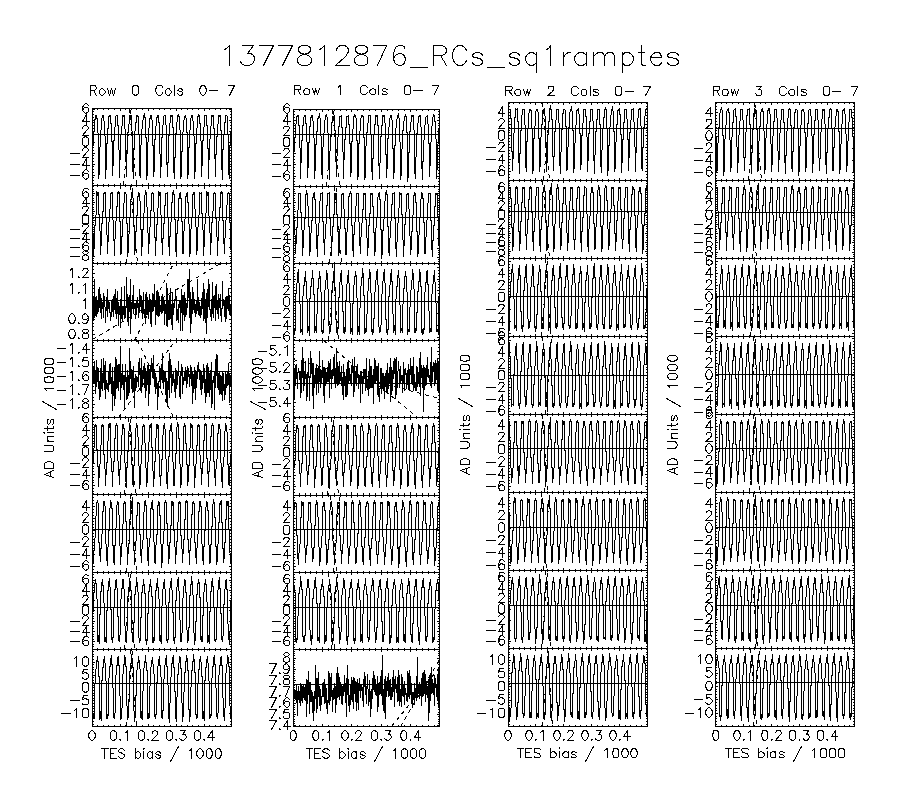
\includegraphics[width=\textwidth]{./images/1377812876_RCs_sq1ramptes_00.png}
\caption{Plot showing response of SQUID amplifier chain to ramp in \TES\ bias current, while \TES\ is superconducting. Data is shown for rows 0--4 for all eight columns. \RC{0}{2}, \RC{0}{3}, \RC{1}{3}, \RC{1}{7} all show no response, only noise (note the change in vertical scale for these row/columns). xxx need to explain units on axes?}
\label{fig:tes-bias-ramp-sc}
\end{figure*}

\begin{figure*}[th]
\centering
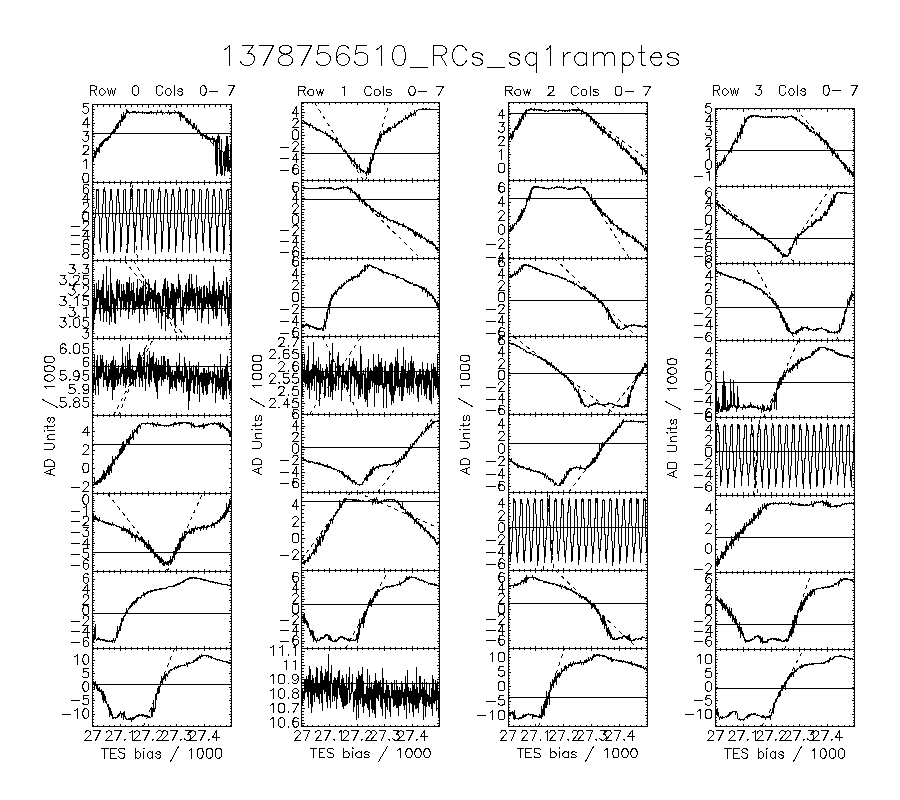
\includegraphics[width=\textwidth]{./images/1378756510_RCs_sq1ramptes_00.png}
\caption{Plot showing response of SQUID amplifier chain to ramp in \TES\ bias current, while \TES\ is biased into transition. The change in applied bias current is the same as in \figref{fig:tes-bias-ramp-sc}.
Data is shown for rows 0--4 for all eight columns.
\RC{0}{2}, \RC{0}{3}, \RC{1}{3}, \RC{1}{7} all show no response, only noise (note the change in vertical scale for these row/columns).
\RC{0}{1}, \RC{2}{5} and \RC{3}{4} all respond as if they were still superconducting (see \figref{fig:tes-bias-ramp-sc}).
The much slower mapping of the $V$-$\phi$ curve indicates a much higher resistance in the \TES\ circuit loop, due to the \TES\ itself starting to go normal.
xxx need to explain units on axes?}
\label{fig:tes-bias-ramp-trans}
\end{figure*}

\begin{figure*}
\centering
\includegraphics{./drawings/ch8-detector-cuts-wafer.pdf}
\caption{
Figure showing detector layout, highlighting which detectors have problems and which are working.
Each detector is labeled (below) with its row/column.
The x and y positions of the detectors on the wafer are also given, given in this thesis in the format X-Y, where X give the x position of the detector (labeled along the bottom) and Y the y position (labeled along the left).
}
\label{fig:detector-cuts-wafer}
\end{figure*}

\begin{figure*}
\centering
\includegraphics{./drawings/ch8-detector-cuts-rc.pdf}
\caption{Figure showing same information as \figref{fig:detector-cuts-wafer}, but organized in term of readout rows/columns. Each detector is labeled (below) with its position on the detector wafer. The rows/columns are labeled on the left and top. Unused row/columns as well as the row/columns used to readout the position of the secondary mirror are also indicated. }
\label{fig:detector-cuts-rc}
\end{figure*}

\section{Readout of Mirror Position}\label{sec:ch8-mirror-readout}

The \Imager\ produces a time-ordered data stream containing the output of each detector as a function of time.
In order to turn this data stream into a video, we must know where the optical system is pointing at all times.
This section desribed how this pointing information is placed directly into the timestream by the \Imager.
It is also necessary to know where each detector is pointed relative to the optical system; this relative detector pointing information is extracted from beam maps, as discussed in \sectionref{s:beam-maps}.

The pointing of the optical system is set by the positions of the two actuators --- \DISP1 and \DISP2 --- that move the secondary mirror.
The actuator control hardware provides two voltage signal which are proportional to the positions of the actuators.
This voltage signal is sent into the \Imager\ cryostat by a pair coaxial cables.
Inside the cryostat two \SI{1}{m} long Phosphur Bronze (xxx exact lakeshore name?) (PhBr) \AWG36 twisted pair wires carry the signal to the focal plane, where the signal is fed into the input coil of a 1st stage \SQUID.
Series resistors (\SI{4.23}{\mega\ohm} for \DISP1, \SI{4.36}{\mega\ohm} for \DISP2) are used at room temperature to reduce the maximum current flowing through the wires to a value appropriate for the 1st stage \SQUID\ input; approximately \SI{2}{\uA}.

This approach synchronizes the actuator position readout with the detector response, and allows both pieces of information to be readout in the same way.

To convert the mirror output current (readout as en electrical current by the readout system) to actuator displacement I moved the mirror actuators in sine-wave patterns with a frequency of \SI{0.1}{\Hz} using 8 different displacement ampitudes.
I fit the resulting output current timestream to a sine waves.
The result are conversion factors of \SI{2.929}{\mm\per\uA} for \DISP1 and \SI{3.024}{\mm\per\uA} for \DISP2.
% see cooldown39/ana_bose_factor.m

To convert actuator displacement to displacements in the farfield of the system, I used the conversion factors produced from \ZEMAX\ listed in \sectionref{sec:ch4-optical-design}.
A \SI{1}{\mm} movement of the actuator produces a change in angle of the secondary mirror of \ang{0.276}; a \ang{1.0} rotation of the secondary mirror displaces the beam of an on-axis detector by \SI{18.35}{\cm} at the far-field focal plane.
The conversion factor between actuator displacement and farfield beam displacement is \SI{5.065}{\cm\per\mm}.

To convert actuator displacements into locations in the farfield, three additional factors should be considered.
First, the cassegrain optical system inverts images that it views, so that a beam from a detector in the lower left of the focal plane (as viewed from behind the detector focal plane) is pointed to the upper right on the farfield image (again as viewed from the system).
Second, tilting the mirror displaces the beams in the same direction as the mirror is tilted; this is easily seen by thinking of the system in transmission, and imagining the way a beam of light is reflected off of a rotated mirror).
Third, the actuators are oriented so that their rotation axes are rotated from horizontal/vertical by \ang{45}.
This all means that --- as viewed from the cryostat --- positive displacements of the \DISP1 actuator shift beams up and to the right, while positive displacements of the \DISP2 actuator shift beams up and to the left.
If we consider an $x$-$y$ coordinate system in the farfield, this means that the $x$ and $y$ displacement of the beams due to mirror movements are calculated as

\begin{equation}
\Delta x = \frac{\sqrt{2}}{2} \left( I_{\DISP1} \times \frac{\SI{2.929}{\mm}}{\SI{1}{\uA}} -
                              I_{\DISP2} \times \frac{\SI{3.024}{\mm}}{\SI{1}{\uA}}  \right) \times
    \frac{\ang{0.276}} {\SI{1}{\mm}} \times
    \frac{\SI{18.35}{\cm}} {\ang{1}}
\end{equation}
\begin{equation}
\Delta y = \frac{\sqrt{2}}{2} \left( I_{\DISP1} \times \frac{\SI{2.929}{\mm}}{\SI{1}{\uA}} +
                              I_{\DISP2} \times \frac{\SI{3.024}{\mm}}{\SI{1}{\uA}}  \right) \times
    \frac{\ang{0.276}} {\SI{1}{\mm}} \times
    \frac{\SI{18.35}{\cm}} {\ang{1}}
\end{equation}


% pivot 14.19 mm behind mirror vertex
% pivot 14mm in front on \BOSE\ attachment point

A natural question is whether cross-talk appears between the actuator readout and the other detectors.
To test this both actuators were moved in a \SI{6}{\Hz} sine-wave pattern over their maximum displacement range of +/- 3.5~mm, while the detectors were bias at \SOC.
Both actuators were moved at the same time, roughly \SI{135}{\degree} out of phase.
The level of crosstalk present can be quantified by performing a least-squares fit of each detector timestream $\vect{d}_{rc}$ to the model
\begin{equation}
	 \vect{d}_{rc} = A_1 \vect{d}_{\DISP1} + A_2 \vect{d}_{\DISP2}.
\end{equation}
Here $\vect{d}_{\DISP1}$ and $\vect{d}_{\DISP2}$ are the measured outputs for each actuator.

To check whether crosstalk from the actuators is a problem for our system, I calculated the crosstalk amplitudes $A_1$ and $A_2$ for each detector twice: once of the first half of the data acquision and once for the second half.
If crosstalk is present to a statistically significant level, a scatterplot of the crosstalk amplitudes for the two halfs of the data acquisition should show signs of correlation.
As can be seen in \figref{fig:ch9-bose-cross}, the points are clustered about the origin, indicating no consistent crosstalk amplitude, and no correlation is apparent.

\begin{figure*}[th]
\centering
\includegraphics[width=\textwidth]{drawings/ch8-bose-cross.pdf}
\caption{
Plot showing crosstalk amplitudes.
The left plot is for \DISP1, the right for \DISP2.
Each actuator was moved +/- \SI{3.5}{\mm} at 6 Hz while the detectors were biased at \SOC.
The best-fit crosstalk amplitude for each actuator and detector were calculated for both the first half and the second half of the data acquisition, and these amplitudes are plotted against each other in these plots.
The lack of correlation in the scatter plots, as well as the clustering around the origin, indicates that any crosstalk present cannot be distinguished from noise in the detectors.
}
\label{fig:ch8-bose-cross}
\end{figure*}

% xxx - I get 500 uW for the load from these four wires (300 K - 1K). Can this be correct? I'm sure I did this calculation in the past and got a much smaller number. Did I screw up in the past? Is today's calculation in error? Am I intercepting this load at 50~K or 4~K, and I forgot about that? Did I use a much longer wire than 1~m? This could be a big cryogenic problem!

\section{Focus Distance}\label{s:focus-distance}

As described in \sectionref{s:optical-design}, the \Imager\ is designed to focus at distances of 16~m -- 30~m (xxx check 2nd distance).
All results described in this chapter were with the \Imager\ configured to focus at 16~m.
To check the actual distance to the target focal plane, beam maps as described in \sectionref{s:beam-maps} were performed with the blackbody source located at different distance from the cryostat.
\figref{fig:beam-vs-distance} shows beam maps for the same detector taken at different distances.
It is clear from this plot that the best focus occurs at \abt{\SI{17}{m}}, and the depth-of-field is approximately xxx~m.

The reasons for the difference from \ZEMAX\ predictions are not understood.
Possibilities include the cryostat being located too close to the primary mirror and the primary (or secondary) mirrors having an incorrect shape.

\section{Beam Maps} \label{sec:ch8-beam-maps}

As discussed in \sectionref{sec:ch4-feedhorn-design}, the \Imager\ feedhorns are predicted to have beams that are circularly symmetric and well-approximated by Gaussians with \FWHM\ of x.xx~cm at the target.
To verify these predictions beam maps were performed by rastering the beams over a small, stationary \SI{1030}{\celsius} blackbody source.

The blackbody source used was an IR Labs xxx\footnote{IRLabs, Inc. Tucson, AZ. USA}.
This source reaches a maximum of \SI{1030}{\celsius} and has apertures ranging in size from x.xx in to x.xx in.
Best results were achieved by covering an area around the blackbody source with Aluminum foil; this eliminated hotspots in the image due to the warmth of the housing of the blackbody source itself.
\figref{xxx} shows a picture of the blackbody source with Aluminum foil mask.

The \Imager\ beams were rastered over the blackbody source by moving one actuator at \SI{6}{\hertz} while the other actuator moved much more slowly at \SI{0.1}{\hertz}.
Scans were taken with the blackbody in two different locations to ensure coverage of the entire subarray.
At each blackbody positions two scans were taken with \DISP1 as the fast actuator and two with \DISP2 as the fast actuator, for a total of eight scans.

For each scan, the data stream for each detector was ``binned'' as described in \sectionref{xxx} to produce a beam map for each detector.
No common mode or polynomial was removed from the timestreams.
Actuator displacements were converted to distances in the far-field using the conversion factors discusssed in \sectionref{sec:ch8-mirror-readout}.
The following 2-D Gaussian allowing for ellipticity was then fit to each beam map:
\begin{multline}
%\begin{split}
  P(x,y) = O + A \exp{ \left[  - \frac{1}{2} \left( \frac{ (x-x_0) \cos{\theta} + (y-y_0) \sin{\theta}}{\sigma_1} \right)^2 
                               - \frac{1}{2} \left( \frac{-(x-x_0) \sin{\theta} + (y-y_0) \cos{\theta}}{\sigma_2} \right)^2
                       \right] }.
%\end{split}
\end{multline}
Here $x$ and $y$ represent the position in the beam map, while $x_0$, $y_0$, $\sigma_1$, $\sigma_2$, $\theta$, $A$, and $O$ are the parameters to be fit.
$O$ represents an overall \DC\ offset in the map level.
Only the points within \SI{3}{\cm} of the map peak were included in the fit.
Beam maps at the edge of the scan were discared, as were beam maps where the fitting routine performed poorly.
The $\theta$, $\sigma_1$, and $\sigma_2$ paremeters were all rationalized so that the conditions $\sigma_1 > \sigma_2$ and $0 < \theta < \ang{180}$ hold.
The beam parmeter across the eight scans were then averaged together to produce final beam maps.
\figref{fig:ch8-beam-summary} summarizes the final fit parameters for all the beams.
The beam ellipticity and angle offset from the $x$-axis are statistically significant.

\figref{fig:ch8-all-beam-maps} shows the final beam maps.
The beams are elliptical, with a mean $\sigma_1 / \sigma_2 = \si{1.6}$.
The mean beam angle is $\ang{70}$ from the $x$-axis.
The beam size \FWHM\ is calculated as
\begin{equation}
  2 \sqrt{2 \ln{2}} \sqrt{\sigma_1 \sigma_2}
\end{equation}
where the prefactor $2 \sqrt{2 \ln{2}}$ converts from the Gaussian parameters $\sigma$ to the gaussian \FWHM.

In \sectionref{sec:ch4-feedhorn-design}, it was shown that the expected \FWHM\ beam width from this measurement is \SI{1.18}{\cm}.
This is very close to the mean of the measured \FWHM\ of the beams.
However, the feedhorn beam should be circular, not strongly elliptical as is observed.
The source of this ellipticity is not known, but three possible explanations are (1) misalignment of the feedhorns with the primary and secondary mirrors (2) diffraction off the aperture stop located in the \SI{50}{\K} radiation sheild (3) errors in fabrication of the mirrors or feedhorns.

The best-fit grid spacing between detector beams in the far field is \SI{1.72}{\cm}.
Using the plate scale extracted from \ZEMAX\ in \sectionref{sec:ch4-optical-design}, this is equivalent to a \SI{2.81}{\mm} detector spacing on the focal plane array.
The design detector spacing, after accounting for predicted thermal contraction of the feedhorn arrays, was \SI{2.730}{\mm}.
Given manufacturing and alignment uncertainties, the closeness of these two numbers is encouraging, and indicates that we have a good understanding of how to map actuator displacements into distances in the farfield of the optical system.

Although the ellipticity of the beams is disappointing, the resolution is very close to target, and the ellipticity is not a barrier to using the system to take video images. The next section describes the algorithm use to turn detector timestreams into videos.

\begin{figure*}[th]
\centering
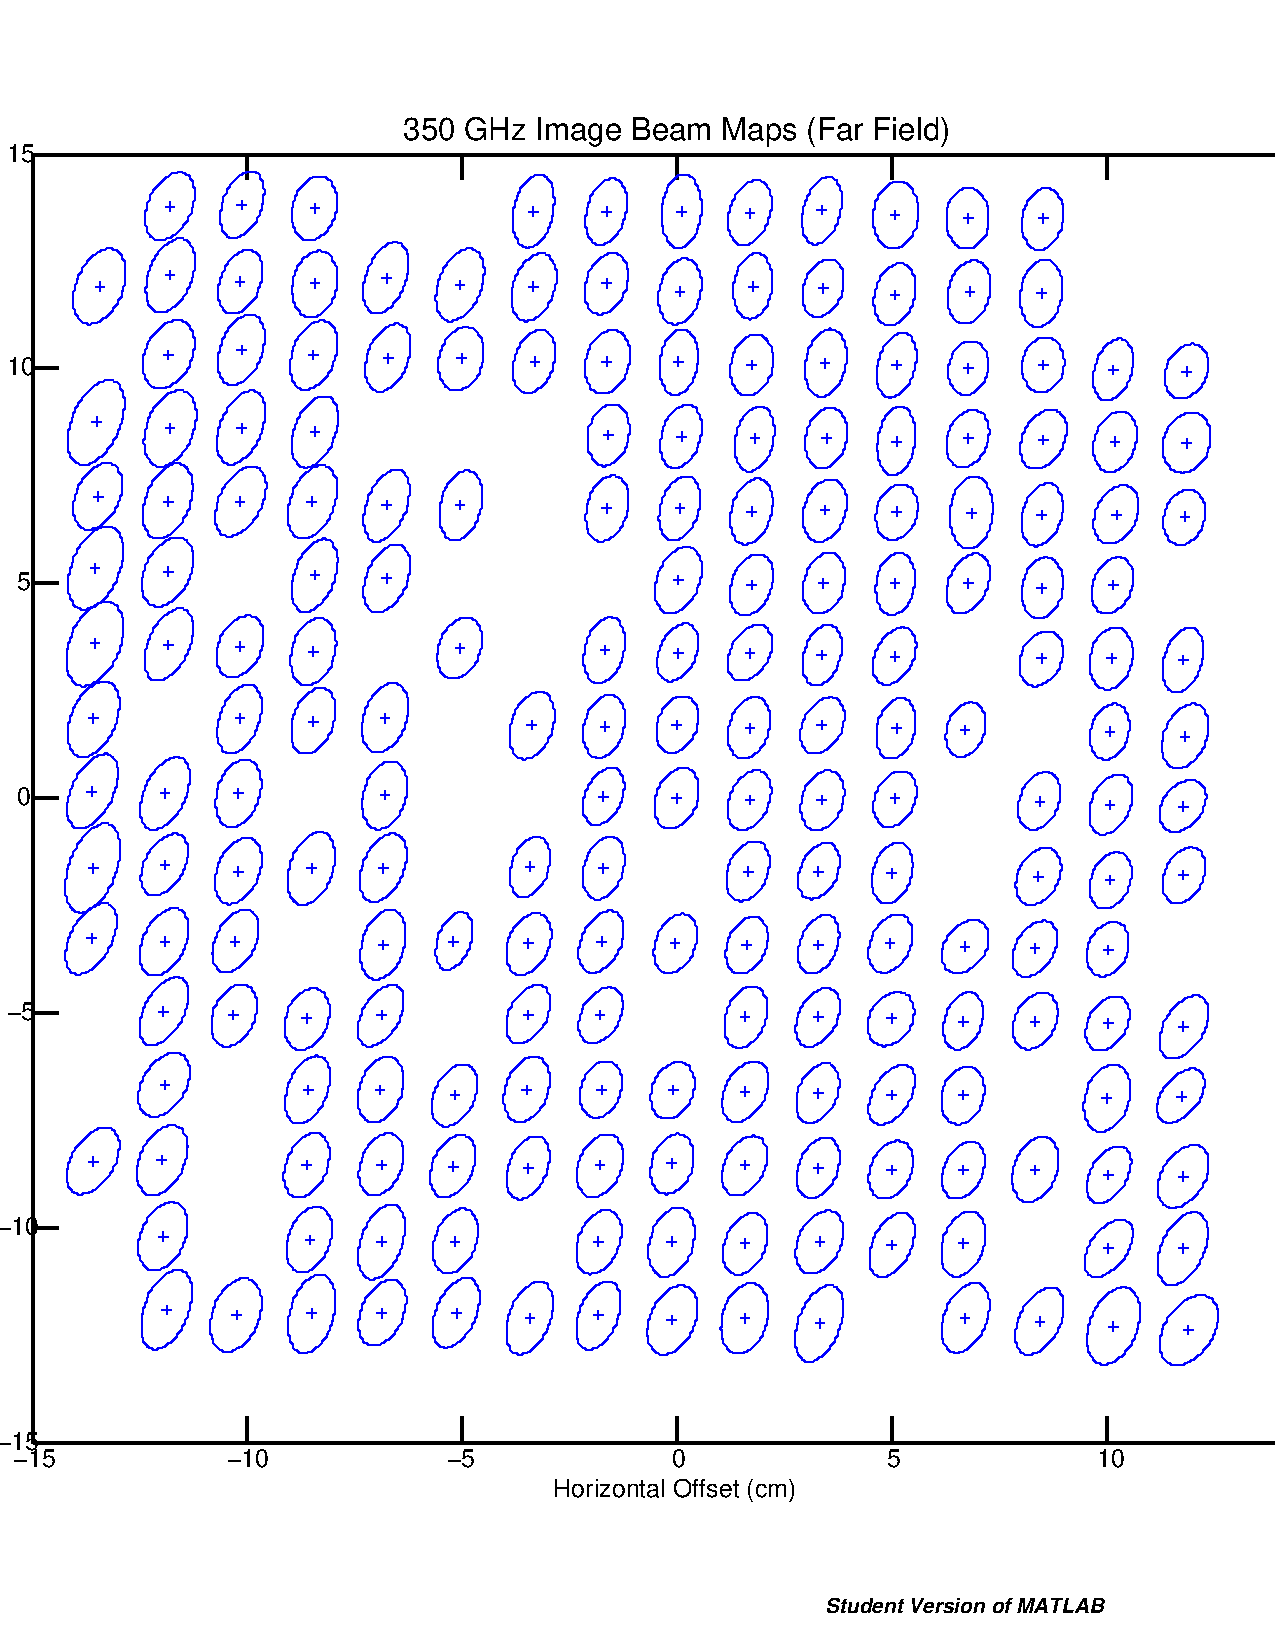
\includegraphics[width=\textwidth]{drawings/ch8-all-beam-maps.pdf}
\caption{
Plot showing final beam maps.
The ellipses represent the full-width-half-maximum of the best-fit 2-D Gaussian for each beam. The beams are elliptical, with a mean $\sigma_1/\sigma_2$ of 1.6, mean beam angle to the $x$-axis of \ang{70}, and beam FWHM of \SI{1.2}{\cm}.
The four grid locations in the extreme upper right corner, as well as the extreme lower left grid point, have no detectors and therefore no beams. All other missing beams are for cut detectors, as discussed in \sectionref{sec:ch8-det-cuts}.
The offset is relative to detector \RCm{18}{4}.
}
\label{fig:ch8-all-beam-maps}
\end{figure*}

\begin{figure*}[th]
\centering
\includegraphics{drawings/ch8-beam-summary.pdf}
\caption{
  Plots summarizing final fit parameters for all beams.
  \textbf{Left Column} Histograms of beam \FWHM\ (defined in text), beam ellipticity (defined as $\sigma_1 / \sigma_2$) and beam angle to $x$-axis.
  \textbf{Right Column} Scatter plots showing correlation of the three parameters with each other. Beam \FWHM\ increases with ellipticity; this is to be expected give it's definition.
}
\label{fig:ch8-beam-summary}
\end{figure*}

\section{Direct Measurement of Distance Scale} \label{sec:ch8-dist-scale}

To check the distance scale described in \sectionref{sec:ch8-mirror-readout}, I placed a styrofoam cooler filled with liquid Nitrogen (LN2) in the farfield of the system and scanned the system over it, using data acquired to create still images.
A sheet of Eccosorb xxx was placed in the cooler to serve as a cold black surface for the system to observe.
Images were acquired of the cooler itself, as well as the cooler with aluminum foils strips taped to the outside.
Each strip was \abt{\SI{4}{\cm}} tall, and the strips were \SI{14.5}{\cm}, \SI{29}{\cm}, and \SI{47.2}{\cm} long.
The interior of the cooler is \SI{67.7}{\cm} wide.
For each image the \FWHM width of the strip --- or the cold space inside the cooler --- was calculated by taking a cut through the still image centered n the strip or cooler.

The result of these measurements is that the \FWHM\ widths were $\SI{13}{\percent} \pm \SI{3}{\percent}$ smaller than the real distances. The source of this discrepancy is not understood.
All distance scales in the remainder of this chapter have been adjusted to account for this discrepancy, so the distace scale on all images is accurate.

% xxx need to comment on implications for beam maps!

% xxx might be nice to have plots for this section, but need to move
% on for now.

% Code: imaging/ana_reso_from_stills.m

\section{Direct Measurement of Resolution}

Using the same cooler filled with LN2 described in \sectionref{sec:ch8-dist-scale}, a dime (diamter \SI{17.91}{\mm}) was taped to the outside of the cooler and a still image was taken.
\figref{fig:xxx} shows the resulting still image, as well as a close-up of the are with the dime.
A 2-D Gaussian was fit to resulting map.
The best-fit Gaussian has ellipticity 1.2 --- smaller than the individual beams, as expected due to convolution with the dime, which is not a point source.
The \FWHM\ of the dime map is \SI{2.0}{\cm}; this is exactly what is expected by convolving a Gaussian with \FWHM\ \SI{1.2}{\cm} with the \SI{1.791}{\cm} dime.
This serves as a confirmation of the beam size determined in \sectionref{sec:ch8-beam-maps}.

\begin{figure*}[th]
\centering
\includegraphics{drawings/ch8-dime-map.pdf}
\caption{
  Plots showing still image of cooler filled with LN2, with a dime (diameter \SI{1.791}{\cm}) taped to it's outside.
  Red is warm, blue cold; the temperature scales are different in the two plots.
  \textbf{Left} The full map of the cooler. The white rectangle shows the area of the detail on the right.
  \textbf{Right} Detail of area within white rectangle: the dime.
  The black ellipse shows the \FWHM of the best-fit ellipse to the map. The ellipticity is \num{1.17}, the FHWM of the principal axes are \SI{1.9}{\cm} and \SI{2.2}{\cm}, for an overall \FWHM\ of $\sqrt{1.9 \times 2.2} = \SI{2.0}{\cm}$.
}
\label{fig:ch8-dime-map}
\end{figure*}

\section{Optical Efficiency} \label{sec:ch8-opt-eff}

We can use the beam map measurements to estimate optical efficiency for all detectors.
The total power falling on a bolometer pointed to position $(x,y)$ in the farfield is given by 
\begin{equation}
  P_{tot} = P_{spill} + \eta_{tot} 2 k_B \Delta \nu \int B(\prime{x} -x, \prime{y} - y) T(x,y) d\prime{x} d\prime{y}.
\end{equation}
Here $P_{spill}$ represents power falling into the detector's feedhorn from any source other than the mirror farfield; this includes both light from inside the cryostat and light making it's way into the feedhorns from outside the cryostat from sources other than the farfield (such as light spilling off of the primary and secondary mirrors.
$P_{spill}$ is assumed to be independent of the position of the secondary mirror and of the temperature distribution in the farfield of the system.
The second term includes all power coming from the farfield; $\eta_{tot}$ is the total optical efficiency from the farfield, $k_B$ is Boltzmann's constant, $\Delta \nu$ is the optical bandwidth of the system, $B$ is the far-field beam pattern (normalized so that it's integral over all space is unity), and $T$ is the farfield temperature distribution.
The factor 2 accounts for the detectors being sensitive to both polarizations, as we assume that the feedhorn's waveguide reduces the system to single-moded detection.

The blackbody source for these measurement was \SI{0.508}{\cm} in diameter and was set to $\SI{1030}{\celsius} = \SI{1303}{\kelvin}$.
We assume that everythig else in the scene was at the same temperature, \SI{295}{\kelvin}.
When the beam is pointed directly at the blackbody source the total power absorbed in the detector is given by
\begin{equation}
  P_{tot,on} = P_{spill} + \eta_{tot} 2 k_B \Delta \nu \left( \SI{1303}{\kelvin} \int_{r \leq \SI{0.508}{\cm}} B(x^{\prime}, y^{\prime}) dx^{\prime} dy^{\prime} + 
                                                       \SI{295}{\kelvin} \int_{r > \SI{0.508}{\cm}} B(x^{\prime}, y^{\prime}) dx^{\prime} dy^{\prime}
                                                \right).
\end{equation}
When the beam is pointed more than a few beam widths away from the blackbody source the total power absorbed in the detector is given by
\begin{equation}
  P_{tot,off} = P_{spill} + \eta_{tot} 2 k_B \Delta \nu \left( \SI{295}{\kelvin} \int_{r \leq \SI{0.508}{\cm}} B(x^{\prime}, y^{\prime}) dx^{\prime} dy^{\prime} + 
                                                       \SI{295}{\kelvin} \int_{r > \SI{0.508}{\cm}} B(x^{\prime}, y^{\prime}) dx^{\prime} dy^{\prime}
                                                \right).
\end{equation}
The difference between these two quantities gives the change in absorbed power moving from on to off the blackbody:
\begin{equation}
  \Delta P_{tot} = \eta_{tot} 2 k_B \Delta \nu \SI{1008}{\kelvin} \int_{r \leq \SI{0.508}{\cm}} B(x^{\prime}, y^{\prime}) dx^{\prime} dy^{\prime}.
\end{equation}

A change in power absorbed in a detector is related to a change in current passing through a detector by the responsivity $s_I{0}$ ($\Delta I = \Delta P s_I(0)$), so that the optical efficiency for a detector is given by
\begin{equation}\label{eqn:opt-eff-from-beams}
  \eta_{tot} = \Delta I \left( s_I(0) 2 k_B \Delta \nu \SI{1008}{\K} \int_{r \leq \SI{0.508}{\cm}} B(x,y) dx dy \right)^{-1}
\end{equation}
In \sectionref{sec:bias-step} $s_I(0)$ was estimated for all detectors.
In this section we have found parameters for estimating the shapes $B$ of the beams for each detector.
The estimated amplitude of the beam maps gives us $\Delta I$.
Given these parameters the integral in \eqnref{eqn:opt-eff-from-beams} can be numerically evaluated, and $\eta_{tot}$ for each detector can be estimated.

\section{Image Processing Algorithm} \label{sec:ch8-algo}

This section describes the algorithm used to turn raw detector timestreams into video images.
The algorithm currently used is very simple, and processes one video frame at a time.

The algorithm steps are as follows:
\begin{enumerate}
\item The  \MCE\ channles containing the actuator displacement (\RCm{32}{5} for \DISP1 and \RCm{32}{6} for \DISP2) are converted to displacements in the farfield as described in \sectionref{sec:ch8-mirror-readout}.
\item Each detectors output is normalized by dividing it by the amplitude of the best-fit guassian from the beam mappings. This accounts for differences in responsivity as well as optical efficiency between detectors. At this point the units for all detector timestreams should be the same, but each detector timestream will have some unknown offset.xxx need to cover this earlier - maybe an optical efficiency section?
\item Determine full range of farfield positions pointed to, accounting for all detectors. Define a \SI{1}{\cm} grid that covers this range in both $x$ and $y$ directions.
\item Divide detector timestreams into sections for each video frame based on \MCE\ readout rate and frequency at which the secondary mirror is rotating.
  If the mirror frequency is $f_m$ and the readout frequency is $f_{ro}$, then each video frame will cover $\lceil f_{ro} / f_{m} \rceil$.
  \textbf{Example:} If the readout frequency is \SI{3125}{\Hz} and the mirror frequency is \SI{6}{\Hz}, then each video frame will cover $\lceil 520.83 \rceil = 521$ samples.
\item For each video frame
  \begin{enumerate}
  \item Perform the following processing for each detector that is not on the cut list described in \sectionref{sec:ch8-det-cuts}:
    \begin{enumerate}
    \item If the detector's timestream shows evidence of glitches, do not include that detector's timestream for this video frame. The simply algorithm used to identify glitches is the following:
      \begin{enumerate}
      \item Calculate the differences between each consequtive value in the timestream.
        If the timestream values are $f_j$, then the differences are $\Delta f_j = f_{j+1} - f_j$.
      \item Calculate the standard deviation of the differences $\Delta f_j$.
      \item If the absolute value of any $\Delta f_j$ is greater than five times the standard deviation, identify this detector as having a glitch, as so to be ignored for this video frame. xxx should say how often this happens, show example of glitch timestream ... maybe show a big plot with all timestreams for a frame, highlighting those with glitches?
      \end{enumerate}
    \item Subtract the median value for this video frame's detector timestream.
          Although crude, this approach does a good job of accounting for the offsets in the detector timestreams, as well as accounting for the common-mode drift described in \sectionref{sec:common-mode}.
    \item If the detector does not have a glitch, determine which image pixel the detector is pointing to at each point in time, using both the pointing position from the actuator readout described in \sectionref{sec:ch8-mirror-readout} and the beam pointing information from \sectionref{sec:ch8-beam-maps}.
    \item Add the detector's value to that pixel for the frame
    \item Keep track of the total number of pixels that have been aded to each pixel
    \end{enumerate}
  \item After each detector has been processed for the frame, divide the value for each pixel by the number of detector that have been used for that pixel
  \end{enumerate}
  \item To improve constrast, all temperature offset values below xxx K are mapped to xxx K, and all temperature values above xxx K were mapped to xxx K.
        Any pixels in the image with no data were assigned a temperature of xxx K.
  \item After all video frames have been processed, convert the resulting 3-dimensional array to a video using \MATLAB's \texttt{VideoWriter} object.
\end{enumerate}

\figref{fig:ch8-single-frames} shows four still images from a vide that was processed according to these rules.
They show the author with a ceramic knife hidden beneath a button-down cotton shirt.
The ceramic knife is visible as a dark area on the left of the shirt.
A darker line running down the center of the shirt is due to the extra layer of cotton backing the buttons; this additional cloth produces more attenuation of the warm light from the body, and so appears cooler.

xxx need to give a URL to where this particular video can be viewed.

xxx need to comment on temperature scale in this image!

\begin{figure*}[th]
\centering
\includegraphics[width=\textwidth]{drawings/ch8-single-frames.pdf}
\caption{
Sample still images from a video taken with the \Imager.
Time proceeds left-to-right and top-to-bottom.
The stills are 20 frames (\SI{3.33}{\s}) apart.
The person in the images is the author.
A ceramic knife hidden beneath a button-down cotton shirt is visible on the left of each image.
The darker line running down the center of the shirt is due to the extra layer of cotton backing the buttons; this additional cloth produces more attenuation of the warm light from the body.
xxx say something about temperature scale once I get it right.}
\label{fig:ch8-single-frames}
\end{figure*}

